\documentclass{article}
\usepackage[T1]{fontenc}
\usepackage{microtype}
\usepackage{graphicx}
\usepackage{booktabs}
\usepackage{amsmath,amssymb}
\usepackage{hyperref}
\usepackage{placeins}
\usepackage{float}
\hypersetup{hypertexnames=false}
\newcommand{\theHalgorithm}{\arabic{algorithm}}
\usepackage[accepted]{icml2023}
\graphicspath{{figures/}}
\setcounter{dbltopnumber}{4}
\setcounter{totalnumber}{6}
\renewcommand{\dbltopfraction}{0.9}
\renewcommand{\textfraction}{0.1}
\setlength{\dblfloatsep}{12pt plus 2pt minus 2pt}
\setlength{\dbltextfloatsep}{14pt plus 2pt minus 2pt}
\setlength{\textfloatsep}{10pt plus 2pt minus 2pt}
\setlength{\floatsep}{8pt plus 2pt minus 2pt}
\setlength{\intextsep}{8pt plus 2pt minus 2pt}
\renewcommand{\arraystretch}{1.08}
\icmltitlerunning{Navigating Movie Taste with Sparse ALS and Genre Priors}
\begin{document}
\raggedbottom
\twocolumn[
\icmltitle{Navigating Movie Taste with Sparse ALS and Genre Priors}
\begin{icmlauthorlist}
\icmlauthor{Ahmed Amin}{aims}
\end{icmlauthorlist}
\icmlaffiliation{aims}{African Institute for Mathematical Sciences (AIMS), South Africa}
\icmlcorrespondingauthor{Ahmed Amin}{aamin@aims.ac.za}
\icmlkeywords{Recommender systems, alternating least squares, MovieLens, cold start}
\vskip 0.3in
]
\printAffiliationsAndNotice{}
\begin{abstract}
This study evaluates a movie recommender on all 32 million MovieLens ratings using a seeded 80/20 train/test split. The system combines alternating least squares (ALS) with movie-genre information. Ten-factor ALS attains a test RMSE of 0.78, compared with 1.06 for the training-mean baseline and 0.86 for a bias-only model. The genre prior yields a modest improvement when ratings are withheld for supported movies, but not for naturally unrated movies. A local application serves recommendations from the saved model, and independent checks reproduce the principal results. Code and supporting materials: \href{https://github.com/ahmedamen1/Recommendation-System-using-ALS-}{GitHub repository}.
\end{abstract}
\section{Introduction}
Movie services offer more films than an individual can browse. Ratings provide a sparse signal of preference because most viewers rate only a small fraction of a catalog. The resulting task is to estimate ratings for unseen films from observed user--item interactions. The evaluation therefore focuses on rating prediction error; lower error alone does not establish better ranking quality or user satisfaction.

Three approaches are evaluated: a training-set mean, a user--movie bias model, and alternating least squares (ALS) with latent user and movie vectors. The factor model captures interaction patterns shared across the dataset and is widely used in recommender systems \citep{koren2009}. Genre information is evaluated as a prior, with particular attention to items with limited rating history. This design distinguishes standard prediction from cold-start settings for users or movies with sparse observations.

The experiments address four questions: the predictive value of personalization over mean and bias baselines; the accuracy--cost trade-off associated with model capacity; the effect of genre information under natural and controlled cold-start definitions; and the feasibility of serving local recommendations to a new user from a saved model. Root mean squared error (RMSE) measures rating prediction, while recommendation examples illustrate model use without constituting a ranking evaluation.

The saved model is also integrated into a local application that accepts ratings, excludes previously rated films, and presents recommendations. The application is a systems demonstration; clicks, ranked-list quality, and user satisfaction were not measured. MovieLens enables comparison on a large public dataset, but the findings apply to this dataset and split and should not be generalized to all viewers without further evaluation.

The study contributes a comparison of these methods using all 32 million MovieLens ratings and a fixed train/test split; analyses of model capacity, user activity, and natural versus controlled cold start; and a local application that fits a new-user profile without retraining movie parameters. Ten-factor ALS attains a test RMSE of 0.78, compared with 1.06 for the training-mean baseline and 0.86 for the bias model. Genre information modestly improves the controlled cold-start result but not the naturally unrated-item result. Because the analysis uses one random split, these estimates are comparative evidence rather than confirmation of gains on future data.

\twocolumn[{
\begin{minipage}{\textwidth}
\section{System Overview and Architecture}
\begin{figure}[H]
\centering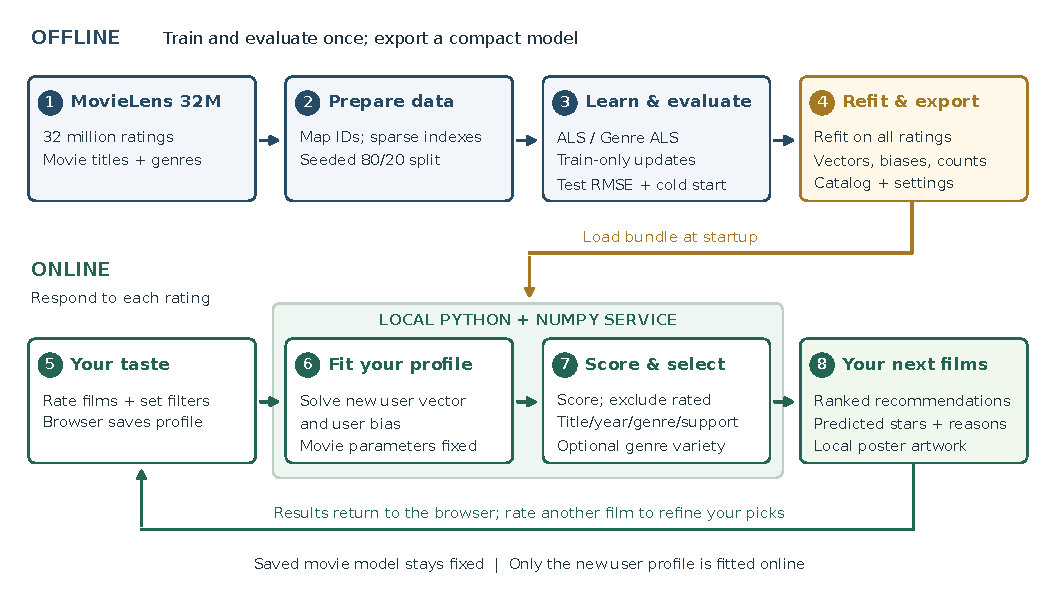
\includegraphics[width=0.94\textwidth]{system_architecture.pdf}
\caption{Full recommendation pipeline. The model is trained and exported once. At run time, a person's ratings update only that user's profile; the saved movie vectors score and filter recommendations.}
\label{fig:architecture}
\end{figure}
\end{minipage}
\vspace{0.8em}
}]
Training is performed once on MovieLens, after which the movie parameters are saved. Figure~\ref{fig:architecture} summarizes the serving pipeline: the local application loads the saved model, estimates a new user's profile from supplied ratings, and scores and filters unrated films. Movie parameters remain fixed during use. An optional genre setting modifies recommendation selection; its effect on recommendation quality and user satisfaction has not been evaluated.


\FloatBarrier
\section{Dataset and Exploratory Analysis}
\subsection{Data and Sparse Storage}
MovieLens 32M contains 32,000,204 ratings from 200,948 users across 87,585 catalog movies \citep{movielens32m,harper2015}. Ratings range from 0.5 to 5 in half-star steps. The release selects users with at least 20 ratings. All observations and catalog movies are retained.

\begin{table}[H]
\caption{Complete dataset and seeded 80/20 split.}
\label{tab:data}\centering\small
\begin{tabular*}{\linewidth}{@{\extracolsep{\fill}}lr}\toprule
Quantity & Count\\\midrule
All ratings & 32,000,204\\
Users & 200,948\\
Catalog movies & 87,585\\
Training ratings & 25,601,250\\
Test ratings & 6,398,954\\
Movies without training ratings & 7,319\\\bottomrule
\end{tabular*}
\end{table}

The observed matrix is 0.18\% dense; a dense float32 representation would need about 65.6 GiB. IDs map to contiguous indices. Chunked loading writes indices, ratings, and split membership to disk-backed arrays. Training entries are indexed in compressed sparse rows by both user and movie. Missing entries are unobserved preferences, not zero ratings.

The catalog includes 3,153 movies without any ratings and 7,319 without training ratings. Every user has training data, with a minimum of eight observations.

\subsection{Distributions}
Four stars is the most frequent rating (Figure~\ref{fig:ratings}). Activity and movie support have long tails (Figure~\ref{fig:degree}), reflecting uneven feedback. Discrete frequency counts produce the horizontal tail bands; the plot alone does not establish a power law.

\begin{figure}[H]
\centering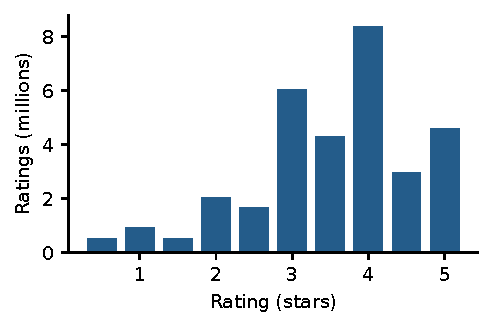
\includegraphics[width=\columnwidth]{rating_distribution.pdf}
\caption{Rating distribution over all 32,000,204 observations.}
\label{fig:ratings}\end{figure}
\begin{figure}[H]
\centering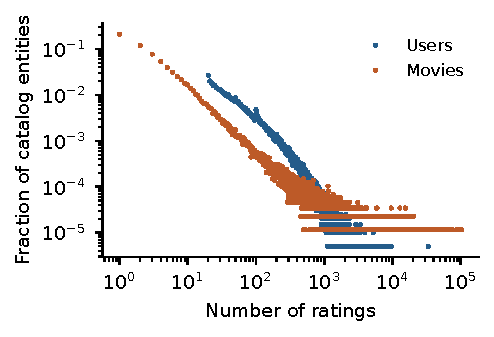
\includegraphics[width=\columnwidth]{degree_distribution.pdf}
\caption{User and movie degrees. Zero-degree movies remain in the denominator but cannot appear on the log axis.}
\label{fig:degree}\end{figure}

\FloatBarrier
\section{Methodology}
The evaluated models are a training-set mean, a bias model, and ALS. User and movie biases represent deviations from the mean, while ALS additionally learns latent vectors whose inner product captures interaction structure. User and movie vectors are $\mathbf{u}_m,\mathbf{v}_n\in\mathbb R^K$, and their biases are $b_m^{(u)},b_n^{(i)}$. $\Omega(m)$ denotes the movies rated by user $m$; $\Pi(n)$ denotes the users who rated movie $n$. Parameters $\lambda$, $\tau$, and $\tau_b$ control the data-fit and shrinkage terms; the implementation names $\tau_b$ as \texttt{gam}.

\subsection{Mean and Bias Baselines}
The mean baseline predicts the training mean. The bias model predicts $\widehat r_{mn}=b_m^{(u)}+b_n^{(i)}$ and maximizes the log joint, up to constants:
\begin{align}
\mathcal L_B={}&-\frac{\lambda}{2}\sum_{(m,n)\in T}(r_{mn}-\widehat r_{mn})^2\nonumber\\
&-\frac{\tau_b}{2}\left[\sum_m(b_m^{(u)})^2+\sum_n(b_n^{(i)})^2\right].
\label{eq:bias-objective}
\end{align}
Setting $\partial\mathcal L_B/\partial b_m^{(u)}=0$ gives
\begin{equation}
b_m^{(u)}=\frac{\lambda\sum_{n\in\Omega(m)}(r_{mn}-b_n^{(i)})}
{\lambda|\Omega(m)|+\tau_b}.
\label{eq:bias}
\end{equation}
The movie update exchanges users and movies, using $\Pi(n)$. Empty rows receive zero bias. No global intercept is fitted ($\mu=0$), so priors shrink biases toward zero.

\subsection{Latent-Factor ALS}
The prediction becomes
\begin{equation}
\widehat r_{mn}=\mathbf{u}_m^{\mathsf T}\mathbf{v}_n+b_m^{(u)}+b_n^{(i)},
\label{eq:prediction}
\end{equation}
with log joint
\begin{align}
\mathcal L={}&-\frac{\lambda}{2}\sum_{(m,n)\in T}(r_{mn}-\widehat r_{mn})^2\nonumber\\
&-\frac{\tau_b}{2}\left[\sum_m(b_m^{(u)})^2+\sum_n(b_n^{(i)})^2\right]\nonumber\\
&-\frac{\tau}{2}\left[\sum_m\mathbf{u}_m^{\mathsf T}\mathbf{u}_m
+\sum_n\mathbf{v}_n^{\mathsf T}\mathbf{v}_n\right].
\label{eq:als}
\end{align}
For fixed movies, update each user bias using Equation~\ref{eq:bias}, subtracting the current interaction in its numerator. Then solve
\begin{align}
\mathbf A_m&=\lambda\sum_{n\in\Omega(m)}\mathbf v_n\mathbf v_n^{\mathsf T}+\tau\mathbf I,\nonumber\\
\mathbf q_m&=\lambda\sum_{n\in\Omega(m)}(r_{mn}-b_m^{(u)}-b_n^{(i)})\mathbf v_n,\nonumber\\
\mathbf A_m\mathbf u_m&=\mathbf q_m.
\label{eq:user-solve}
\end{align}
Movie updates are symmetric. Each sweep updates users, then movies. Since $\tau>0$, the normal matrix is positive definite; the implementation solves the system without explicitly inverting it.

Exact block updates increase $\mathcal L$ despite joint nonconvexity. The code minimizes and plots $\mathcal J=-\mathcal L$, so its objective decreases. Factors start from Gaussian draws with standard deviation 0.1 and seed 42. Effective penalties are $\tau_b/\lambda$ and $\tau/\lambda$; changing $\lambda$ changes both.

\subsection{Genre Prior}
Let $\mathbf x_n\in\mathbb R^{19}$ assign $1/\sqrt{g_n}$ to each of movie $n$'s $g_n$ genres, or zero if none are listed. Rows of $\mathbf F$ are genre vectors; the prior mean is $\mathbf F^{\mathsf T}\mathbf x_n$. For movies $W$ with training ratings, replace the movie penalty in Equation~\ref{eq:als} to obtain
\begin{align}
\mathcal L_G={}&-\frac{\lambda}{2}\sum_T(r_{mn}-\widehat r_{mn})^2\nonumber\\
&-\frac{\tau_b}{2}\left[\sum_m(b_m^{(u)})^2+\sum_n(b_n^{(i)})^2\right]\nonumber\\
&-\frac{\tau}{2}\sum_m\|\mathbf u_m\|^2
-\frac{\tau}{2}\sum_{n\in W}\|\mathbf v_n-\mathbf F^{\mathsf T}\mathbf x_n\|^2\nonumber\\
&-\frac{\eta}{2}\|\mathbf F\|_F^2.
\label{eq:genre}
\end{align}
The movie-vector equation gains $\tau\mathbf F^{\mathsf T}\mathbf x_n$ on its right side. With rows of $\mathbf X_W$ and $\mathbf V_W$ equal to $\mathbf x_n^{\mathsf T}$ and $\mathbf v_n^{\mathsf T}$, update genres through
\begin{equation}
(\tau\mathbf X_W^{\mathsf T}\mathbf X_W+\eta\mathbf I)\mathbf F
=\tau\mathbf X_W^{\mathsf T}\mathbf V_W.
\label{eq:feature-solve}
\end{equation}
Only warm movies enter this solve. A movie without training ratings receives $b_n^{(i)}=0$ and $\mathbf v_n=\mathbf F^{\mathsf T}\mathbf x_n$. New users still require ratings or a fallback.

\section{Experimental Setup and Implementation}
\subsection{Compiled Updates}
Numba compiles the reference accumulations and linear solves. Users update independently with movies fixed, followed by the movie phase; parallel iterations write separate parameter rows \citep{numbaParallel}. Ratings use float32, while parameters and accumulated errors use float64. Batched evaluation avoids allocating a ratings-by-factors matrix. Per-sweep complexity is $O(|T|K^2+(M+N)K^3)$.

The recorded Linux run used Python 3.13, NumPy 2.1, and Numba 0.61, with two Numba threads and one BLAS thread. Table~\ref{tab:benchmark} compares identical starting parameters after compilation warmup and verifies agreement with the reference. Compilation supplies the main speedup; parallel scheduling adds overhead on this bounded workload.

\begin{table}[H]
\caption{One user-side update on 64,301 ratings, $K=10$. Medians of three timings after warmup.}
\label{tab:benchmark}\centering\small\begin{tabular*}{\linewidth}{@{\extracolsep{\fill}}lrr}
\toprule
Method & Median (ms) & Speedup \\
\midrule
Python reference & 811.34 & 1.00$\times$ \\
Numba serial & 14.85 & 54.64$\times$ \\
Numba parallel & 15.34 & 52.91$\times$ \\
\bottomrule
\end{tabular*}

\end{table}

\subsection{Evaluation Protocol}
Seed 42 assigns each rating to training with probability 0.8 (Table~\ref{tab:data}). Updates use training data only. There is no validation set. Test RMSE is monitored, but factor models retain sweep 20 without early stopping or checkpoint selection.

The baseline fixes $K=10$, $\lambda=0.01$, $\tau_b=0.001$, and $\tau=0.1$. Comparisons change one setting: $K=20$, $\tau=0.01$, $\tau=1$, or $\lambda=0.1$. Genre ALS adds $\eta=0.1$. Baseline settings also supply the genre and full-data refits; separate $K=2$ models produce the embeddings.

For test observations $S$, evaluate unclipped predictions using
\begin{equation}
\operatorname{RMSE}(S)=\sqrt{\frac{1}{|S|}\sum_{(m,n)\in S}(r_{mn}-\widehat r_{mn})^2}.
\end{equation}
Metrics are reported to two decimals; full-precision values remain in the result CSVs. Hyperparameters retain their exact values. The monitored test set is not an untouched final holdout.

\subsection{Bias-History Correction}
The bias run contains eight updates followed by twenty more with a restarted counter. Independent fitting reproduces all 28 updates. Figure~\ref{fig:bias} corrects only the cumulative-update axis; factor models still use 20 sweeps.

\begin{figure}[H]
\centering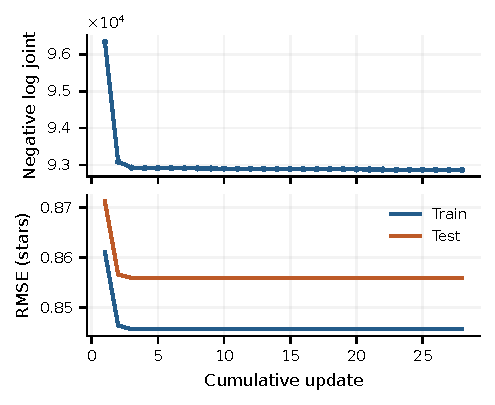
\includegraphics[width=\columnwidth]{bias_learning_curves.pdf}
\caption{Bias fitting over 28 verified updates. The plotted objective is the negative log joint, $\mathcal J_B=-\mathcal L_B$.}
\label{fig:bias}\end{figure}

\section{Results and Discussion}
\subsection{Biases and Factors}
Test RMSE falls from 1.06 for the training mean to 0.86 for biases and 0.78 for ten-factor ALS (Table~\ref{tab:results}). Interactions therefore improve substantially on user and movie offsets. Most improvement occurs in the first few sweeps, with little change near the fixed final checkpoint (Figure~\ref{fig:als}).

\begin{table}[H]
\caption{Final test RMSE. The ALS variants tie at two-decimal precision; this does not imply identical predictions.}
\label{tab:results}\centering\small\begin{tabular*}{\linewidth}{@{\extracolsep{\fill}}lrr}
\toprule
Model & Updates & Test RMSE \\
\midrule
Training mean & -- & 1.06 \\
Biases only & 28 & 0.86 \\
ALS, $K=10$ & 20 & 0.78 \\
ALS, $K=20$ & 20 & 0.78 \\
Genre ALS, $K=10$ & 20 & 0.78 \\
\bottomrule
\end{tabular*}

\end{table}
\begin{figure}[H]
\centering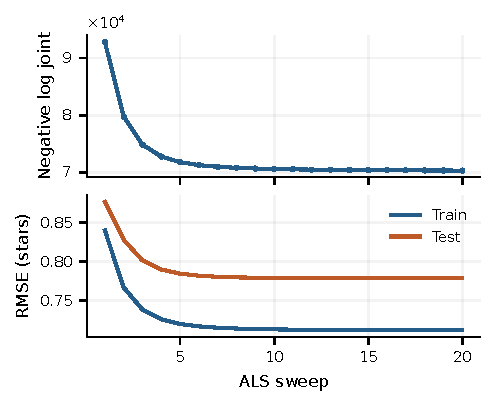
\includegraphics[width=\columnwidth]{practical3_learning_curves.pdf}
\caption{Ten-factor ALS: negative log joint decreases and train/test errors approach a plateau.}
\label{fig:als}\end{figure}

\subsection{Capacity and Regularization}
Twenty factors reduce training RMSE from 0.71 to 0.66, while both test errors round to 0.78. The small unrounded test gain costs 2.22 times more fitting time (Figure~\ref{fig:capacity}; Table~\ref{tab:experiments}).

\begin{figure}[H]
\centering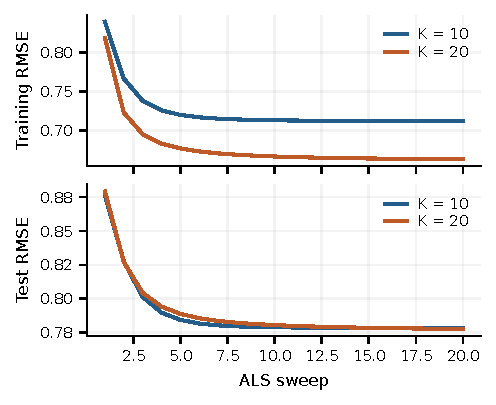
\includegraphics[width=\columnwidth]{capacity_comparison.pdf}
\caption{Training and test RMSE by factor count. Higher capacity lowers training error with little test improvement.}
\label{fig:capacity}\end{figure}
\begin{table}[H]
\caption{ALS comparisons with $\tau_b=0.001$ and 20 sweeps. Train and test columns report RMSE; times include training and evaluation.}
\label{tab:experiments}\centering\small\setlength{\tabcolsep}{2pt}\begin{tabular*}{\linewidth}{@{\extracolsep{\fill}}lrrrrrr}
\toprule
Setting & $K$ & $\lambda$ & $\tau$ & Train & Test & Time (s) \\
\midrule
Baseline & 10 & 0.01 & 0.1 & 0.71 & 0.78 & 190.48 \\
$K=20$ & 20 & 0.01 & 0.1 & 0.66 & 0.78 & 423.75 \\
$\tau=0.01$ & 10 & 0.01 & 0.01 & 0.70 & 0.79 & 198.06 \\
$\tau=1$ & 10 & 0.01 & 1 & 0.77 & 0.80 & 184.43 \\
$\lambda=0.1$ & 10 & 0.1 & 0.1 & 0.70 & 0.79 & 184.50 \\
\bottomrule
\end{tabular*}

\end{table}

Weakening $\tau$ to 0.01 or raising $\lambda$ to 0.1 improves training fit but worsens test RMSE to 0.79. Their test errors reach minima at sweep 12, then rise while the training objective decreases: evidence of overfitting. Raising $\lambda$ also weakens the effective bias penalty. Stronger $\tau=1$ worsens both training and test fit.

Twenty factors help the most-active users but worsen both lower-activity groups (Table~\ref{tab:activity}). The 100+ group contributes most test observations and drives the aggregate gain. Less-active users provide less evidence for larger vectors.

\begin{table}[H]
\caption{Test RMSE by user training activity, using identical observations for both models.}
\label{tab:activity}\centering\small\begin{tabular*}{\linewidth}{@{\extracolsep{\fill}}lrrr}
\toprule
Train ratings & Test rows & $K=10$ & $K=20$ \\
\midrule
1--19 & 101,076 & 0.93 & 0.95 \\
20--99 & 1,365,017 & 0.83 & 0.85 \\
100+ & 4,932,861 & 0.76 & 0.75 \\
\bottomrule
\end{tabular*}

\end{table}

\subsection{Genre Prior and Cold Start}
Genre ALS has training RMSE 0.71 and test RMSE 0.78. Its unrounded test improvement over ten-factor ALS is only 0.10\%; one split does not establish significance. Test error reaches a shallow minimum at sweep 15, but the retained model remains sweep 20 (Figure~\ref{fig:genre}).

\begin{figure}[H]
\centering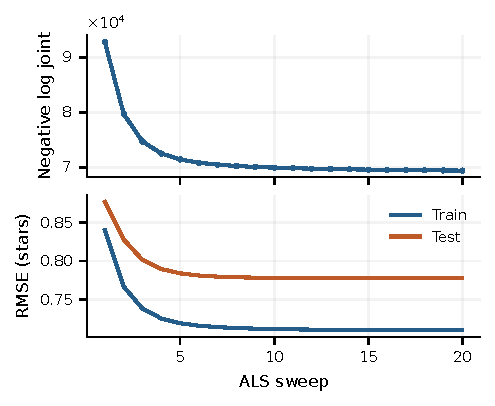
\includegraphics[width=\columnwidth]{genre_learning_curves.pdf}
\caption{Genre ALS: negative log joint decreases; test RMSE has a shallow minimum at sweep 15.}
\label{fig:genre}\end{figure}
\begin{table}[H]
\caption{Warm-user test groups. The controlled study withholds training ratings for 1,063 supported movies.}
\label{tab:cold}\centering\small\begin{tabular*}{\linewidth}{@{\extracolsep{\fill}}lrrr}
\toprule
Test group & Ratings & ALS & Genre ALS \\
\midrule
Warm items & 6,394,233 & 0.78 & 0.78 \\
Natural cold items & 4,721 & 1.03 & 1.04 \\
Controlled cold items & 329,121 & 0.99 & 0.97 \\
\bottomrule
\end{tabular*}

\end{table}

For naturally cold items, genres worsen RMSE from 1.03 to 1.04 (Table~\ref{tab:cold}). This group contains only 4,721 test ratings, so its effect on aggregate error is small.

The controlled study selects 5\% of movies with at least 20 training ratings (seed 43), removes their training observations, and refits both models. Evaluation uses their test ratings from users who retain training data. Independent reconstruction verifies 1,063 movies and 329,121 test observations. Recorded RMSE improves from 0.99 to 0.97 with genres, a 2.22\% reduction calculated before rounding.

Naturally unsupported and deliberately withheld movies are different populations. These results do not show that genres always improve cold start; the controlled study also lacks saved checkpoints for independent error recomputation.

\subsection{Two-Dimensional Fits}
Figures~\ref{fig:movies2d} and~\ref{fig:genres2d} show models trained directly with $K=2$. Nearby Star Wars films and the Crime/Mystery genre pair illustrate learned relationships, but the axes have no intrinsic meaning because joint rotation or reflection preserves dot products. Both test RMSEs round to 0.81, above the main models.

\begin{figure}[H]
\centering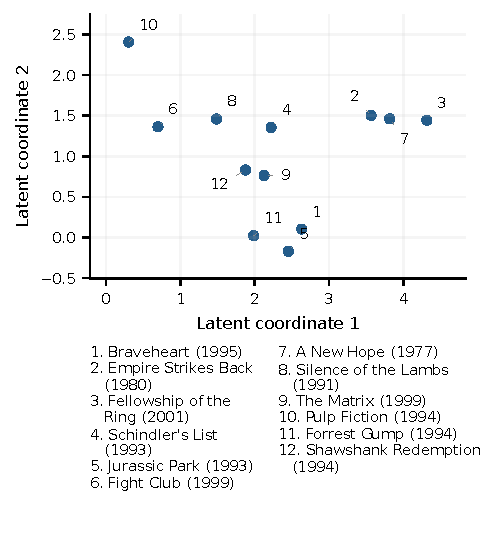
\includegraphics[width=\columnwidth]{movies_2d.pdf}
\caption{Direct two-factor movie fit. Numbers identify twelve frequently rated films; the key uses shortened titles.}
\label{fig:movies2d}\end{figure}
\begin{figure}[H]
\centering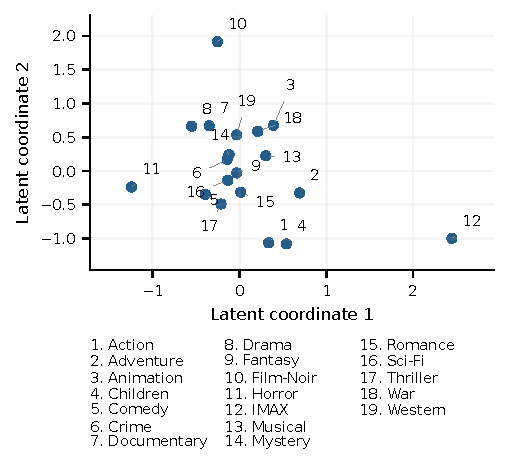
\includegraphics[width=\columnwidth]{genres_2d.pdf}
\caption{Direct two-factor genre fit. Labels are offset without moving the learned coordinates.}
\label{fig:genres2d}\end{figure}
\FloatBarrier

\section{Recommendation Application and Verification}
\subsection{New-User Recommendations}
After evaluation, both models are refitted on all ratings for 20 sweeps. Their training RMSEs round to 0.72; these are not test scores. For a new user $m$, let $\mathbf D$ have rows $[\mathbf v_n^{\mathsf T},1]$, $y_n=r_{mn}-b_n^{(i)}$, and $\boldsymbol\theta=[\mathbf u_m^{\mathsf T},b_m^{(u)}]^{\mathsf T}$. With movie parameters fixed, solve
\begin{equation}
[\lambda\mathbf D^{\mathsf T}\mathbf D+\operatorname{diag}(\tau,\ldots,\tau,\tau_b)]\boldsymbol\theta
=\lambda\mathbf D^{\mathsf T}\mathbf y.
\label{eq:new-user}
\end{equation}
Rank unrated movies by $\mathbf u_m^{\mathsf T}\mathbf v_n+b_n^{(i)}$; the user bias is constant. The practical's alternative weight $0.05b_n^{(i)}$ changes ranking, not predicted stars.



The other Lord of the Rings films lead the supported list (Table~\ref{tab:recommendations}). Allowing single-rating movies instead produces raw predictions as high as 6.31, exposing weakly supported extrapolation. The dashboard filters support and clips displayed stars to 0.5--5; ranking uses raw scores.

\begin{table}[H]
\caption{Genre-model recommendations after rating The Fellowship of the Ring five stars; support $\geq100$.}
\label{tab:recommendations}\centering\small\begin{tabular*}{\linewidth}{@{\extracolsep{\fill}}lrr}
\toprule
Recommended movie & Prediction & Support \\
\midrule
The Return of the King (2003) & 4.71 & 67,449 \\
The Two Towers (2002) & 4.67 & 67,463 \\
A New Hope (1977) & 4.30 & 85,010 \\
The Empire Strikes Back (1980) & 4.27 & 72,151 \\
Return of the Jedi (1983) & 4.16 & 67,496 \\
\bottomrule
\end{tabular*}

\end{table}

\subsection{Movie-Vector Norms}
Table~\ref{tab:polarization} lists the largest norms among movies with at least 100 ratings. Dumb \& Dumber leads with norm 7.37 and rating standard deviation 1.20. Norms depend on factor scale and regularization, not just rating dispersion.

\begin{table}[H]
\caption{Largest supported movie-vector norms. SD denotes rating standard deviation over all observations.}
\label{tab:polarization}\centering\small\setlength{\tabcolsep}{3pt}\begin{tabular*}{\linewidth}{@{\extracolsep{\fill}}p{0.52\linewidth}rrr}
\toprule
Movie & Norm & SD & Support \\
\midrule
Dumb \& Dumber (1994) & 7.37 & 1.20 & 36,802 \\
The Return of the King (2003) & 6.54 & 1.01 & 67,449 \\
The Two Towers (2002) & 6.45 & 1.00 & 67,463 \\
The Fellowship of the Ring (2001) & 6.44 & 1.01 & 73,122 \\
Deathly Hallows: Part 1 (2010) & 6.28 & 1.02 & 20,969 \\
\bottomrule
\end{tabular*}

\end{table}




\subsection{Independent Checks}
\label{sec:verification}
Independent checks verify data hashes and split membership and reproduce saved models' RMSEs, objectives, bias updates, activity groups, and recommendations. Controlled cold-start membership is verified, but its fitted checkpoints were not exported. Two-dimensional coordinates are available, but their checkpoints are also absent.

\subsection{Limitations}
A random rating split evaluates predictions for users and movies represented in the training data and does not establish performance on future ratings. The test set was monitored during development and is therefore not an untouched final holdout. Results cover one random split; neither multiple-seed uncertainty estimates, ranking benchmarks, nor user studies were obtained. Full-precision results and verification scripts accompany the report.

\section{Conclusion}
Sparse storage and compiled updates support ALS fitting on all 32 million ratings. Ten-factor ALS attains lower test RMSE than the mean and bias-only baselines. Increasing the factor count raises fitting time with little aggregate test improvement and degrades results for lower-activity users. Genre information improves the controlled cold-start estimate but not the estimate for naturally unrated movies. The local application demonstrates recommendation serving from saved movie parameters without retraining. Future work should evaluate temporally held-out ratings, ranking metrics, and user outcomes.

\FloatBarrier
\section*{Acknowledgments}
This project was developed as part of Prof. Ulrich Paquet's course. The author gratefully acknowledges his supervision and guidance and thanks the teaching assistant team for their support.
{\interlinepenalty=10000
\bibliography{references}
\bibliographystyle{icml2023}
}
\end{document}
